\documentclass{article}
% \usepackage[utf8x]{inputenc}
\usepackage{microtype}
%\usepackage[icelandic]{babel}
\usepackage{amsfonts}
\usepackage{amssymb}

\usepackage[T1]{fontenc}
\usepackage[utf8]{inputenc}
\usepackage{lmodern}

\usepackage{verbatim}
\usepackage{booktabs}
\usepackage{graphicx}
\usepackage{amsmath}
\usepackage{tcolorbox}
\usepackage{subcaption}
\usepackage{hyperref}
\usepackage{parskip}

\usepackage{chngcntr}

% \usepackage[margin=3cm]{geometry}
\usepackage{graphicx,wrapfig}

% \usepackage[round]{natbib}   % omit 'round' option if you prefer square brackets
% \bibliographystyle{plainnat}
% \usepackage[bibstyle=numeric,citestyle=authoryear,backend=biber]{biblatex}

% Default fixed font does not support bold face
\DeclareFixedFont{\ttb}{T1}{txtt}{bx}{n}{12} % for bold
\DeclareFixedFont{\ttm}{T1}{txtt}{m}{n}{12}  % for normalf

% Custom colors
\usepackage{color}
\definecolor{deepblues}{rgb}{0,0,0.5}
\definecolor{deepred}{rgb}{0.6,0,0}
\definecolor{deepgreen}{rgb}{0,0.5,0}

\usepackage{listings}

% Python style for highlighting
\newcommand\pythonstyle{\lstset{
language=Python,
basicstyle=\ttm,
otherkeywords={self},             % Add keywords here
keywordstyle=\ttb\color{deepblue},
emph={MyClass,__init__},          % Custom highlighting
emphstyle=\ttb\color{deepred},    % Custom highlighting style
stringstyle=\color{deepgreen},
frame=tb,                         % Any extra options here
showstringspaces=false            %
}}

% Python environment
\lstnewenvironment{python}[1][]
{
\pythonstyle
\lstset{#1}
}
{}

% Python for external files
\newcommand\pythonexternal[2][]{{
\pythonstyle
\lstinputlisting[#1]{#2}}}

% Python for inline
\newcommand\pythoninline[1]{{\pythonstyle\lstinline!#1!}}



\setlength{\columnsep}{1cm}
\setlength\parindent{0pt}

\title{Synthesis of Face Images Using Generative Algorithms.}

\author{René Haas \\ Supervisor: Stella Grasshof}



\begin{document}

\maketitle
\tableofcontents
\newpage


\section{Introduction}

A distinction between machine learning models are that between \emph{disciminative} and \emph{generative} models. In discriminative models we assign a label to a datapoint. For example given an image, which category does it belong to - is it a cat or a horse? Generative models however tries to approximate samples from a data distribution from a learned distribution.

In this research project we will explore different generative models on the domain of face synthesis. We can distinguish two main types of generative models: likelihood based models, which include Variational Autoencoders (VAEs) and implicit models such as Generative Adversarial Networks (GANs)\cite{vqvae2}.

In this project we will implement Principal Component Analysis(PCA) a VAE and a GAN and compare the results of generating faces with these three methods.

We will start in the next
exploring different architectural implementation along the way.

The expected outcome of theis project is theree folde

1) gaining an overview of modern generative models trhough a literature survery. Here we will review recent litterature and explore there different recent  architectural implementation of VAEs and GANS. We will provide the nessecary theory along the way. Wwith we will do in the next section

2) gain practical understanding by implementing versions of the different models and training them two different datasets.

3) Finally we will Furthermore we will explore the latent space of pre trained models and show that we can use these to do state-of-the-art face synthesis and semantic face editing.

\chapter{Theory}


\section{Inception Score}
\url{https://machinelearningmastery.com/how-to-implement-the-inception-score-from-scratch-for-evaluating-generated-images/}


\section{Principal Component Analasyis. }

\section{Probabilistic models}
We assume that the observed variable $\mathbf{x}$ is a sample from the true distribution $p^*(\mathbf{x})$.\cite{vaeintro} Out goal is to approximate the true distribution with a model such that

\begin{align}
  p_\theta(\mathbf{x})\approx p^*(\mathbf{x})
\end{align}

Now, how do we ego about actually modeling this distribution $p_\theta(\mathbf{x})$?. We can use Neural networks to parametrize the distribution.

The log-probability of the data is
\begin{align}
  \log p_\theta(\mathcal{X}) = \sum_{\mathbf{x}\in\mathcal{X}} p_\theta(\mathbf{x})
\end{align}

Maximization of the log-likelihood is equivalent to minimizing the KullBack-Leibler divergence.

The KullBack-Leibler divergence is given by

\begin{align}
D_{\text{KL}}(p_\theta,q_\phi) = -\sum_{\mathbf{x}\in\mathcal{X}}p_\theta(\mathbf{x})\log \frac{q_\phi(\mathbf{x})}{p_\theta(\mathbf{x})}
\end{align}

% \section{Survey}

\section{Variational Autoencoders.}
The encoder network models$p_\theta(\mathbf{z}|\mathbf{x})$ while the encoder network models $p_\theta(\mathbf{x}|\mathbf{z})$


\section{GANs}

The premise of GANs is to play minmax game between two competing neural networks. We simultaneously train a discriminator $D$ and a generator $G$.
The discriminator $D$ is a binary classifier whose objective is classify whether a show example image is coming from the data distribution $p_D$ or from the generated $p_G$ distribution.

The original value function,proposed in 2014 by Ian Goodfellow et al.\cite{gan} is given by
\begin{align}
\mathcal{L} = \min_G \max_D V(D,G))=\mathbb{E}_{\mathbf{x}\sim p_{\text{data}}(\mathbf{x})}
\left[\log D(\mathbf(x))]\right]+
\mathbb{E}_{\mathbf{z}\sim p_{\mathbf{z}}(\mathbf{z})}
\left[\log (1-D(G(\mathbf(z)))]\right]
\end{align}
Here the $G$ tries to minimize $\mathcal{L}$ while the $D$ tries to maximize it.

Since $D$ is taking a data point (image) $\mathbf{x}\in X$ and giving the probability that image is real or generated, it is a mapping $D:X \to (0,1)$.

We define the generator as to depend on a latent variable $\mathcal{z}\in Z$ such that $G(\mathcal{z})$ is a mapping $G:Z\to X$.




% \paragraph{Face Aging}
% \textit{Face Aging With Conditional Generative Adversarial Networks} (2017) \cite{faceaging}

% \section{3D Reconstruction}
%
% \textit{Projective Structure from Facial Motion}(2017)\cite{ProjectiveStructure}
%
% \textit{Apathy is the Root of all Expressions}(2017)\cite{apathy}
%
% In the paper \textit{"Large Pose 3D Face Reconstruction from a Single Image via Direct Volumetric CNN Regression"}(2017)\cite{largepose}
% the authors used a Convolutional Neural Network to reconstruct the 3D facial geometry from just a single image. The model work under arbitrary poses
% and expressions and without the need of a 3D Morphable Model.

\newpage
\section{Training our own models.} \label{training}

In this section we will present out results with training our own models. We will start by presenting the data sets used and then go on to present the results of running the  PCA, VAE and DCGAN models on the data.

\subsection{Data sets}
In the following we will use two different datasets which we will refer to as the \emph{Caltech} and the  \emph{FFHQ} dataset respectively. 1)  \emph{Caltech} \footnote{Available at \url{http://www.vision.caltech.edu/html-files/archive.html}} which consists of "450 frontal face images of 27 or so unique people." and 2) \emph{FFHQ}\footnote{Available at \url{https://github.com/NVlabs/ffhq-dataset}} Here we use the 5000 of the provided thumbnails of resolution 128x128.

The FFHQ dataset is already preprocessed such that the faces are aligned and the images are of the same dimensions. For Caltech however we need to do this preprocessing manually.

In the Github repository for this project we provide code to download both datasets with additional preprocessing  (face extraction and resizing to 128x128) of the Caltech dataset.\footnote{Code is available here: \url{https://github.com/renhaa/faces/blob/master/DownloadDataset.ipynb}}

In Figure \ref{rawdata} we see a random sample of the processed images from the Caltech \ref{raw-caltech} and FFHQ \ref{raw-ffhq} datasets respectively.

\begin{figure}[h!]
    \centering
    \begin{subfigure}[b]{0.45\textwidth}
        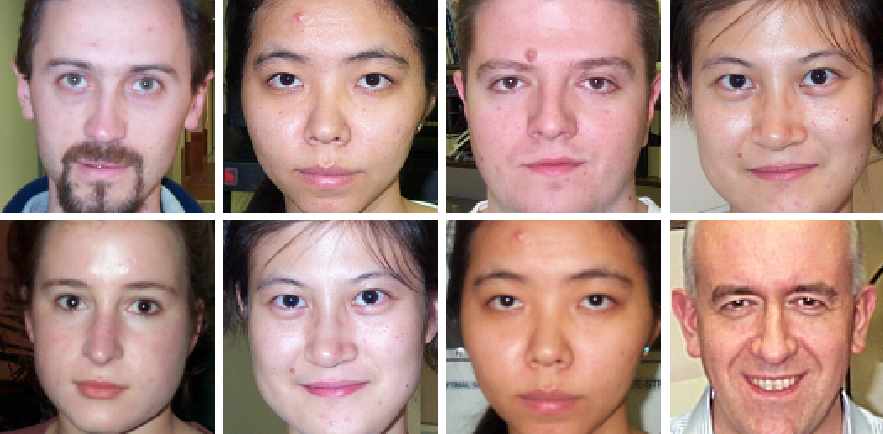
\includegraphics[width=\textwidth]{fig/data/caltech}
        \caption{Caltech dataset}
        \label{raw-caltech}
    \end{subfigure}
    ~
    \begin{subfigure}[b]{0.45\textwidth}
        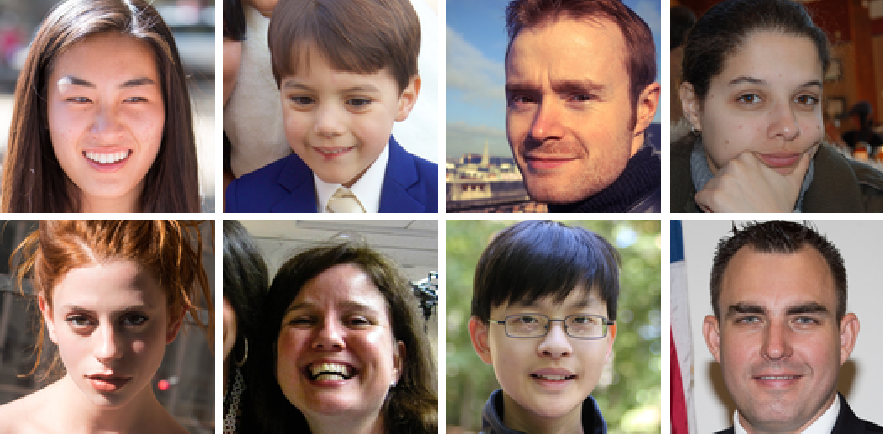
\includegraphics[width=\textwidth]{fig/data/ffhq}
        \caption{FFHQ dataset}
        \label{raw-ffhq}
    \end{subfigure}

    \caption{The raw data from the Caltech and FFHQ datasets respectively.}
    \label{rawdata}
\end{figure}

The FFHQ dataset have a much higher variation than the Caltech dataset, having samples of faces across all ages poses and ethnicities while the Caltech dataset is more limited having the same 27 people facing directly at the camera.

In the following we will use both the colored version of the datasets and for some models we will use a black and white version.

\subsection{Principal Component Analysis}

Here we present our results of doing Principal Component analysis on the FFHQ dataset.

In the process of constructing the design matrix we simply flatten each of the 120x120x3 dimensional color images to 49152 dimensional flat vectors. The normalize these vectors to zero mean and unit variance using\\ {\tt sklearn.preprocessing.StandardScaler} and calulate the eigenfaces with {\tt sklearn.decomposition.PCA}\footnote{The code is available here: \url{https://github.com/renhaa/faces/blob/master/PCA.ipynb}}

In Figure \ref{eigenfacehere} we see the first 8 eigenfaces. In Figure. \ref{eigenface} in the appendix there is a larger version of this figure. We note that the generated faces from the Caltech dataset have some artifacts in the form of shadowy lines across the faces. This are not present in the faces generated from training on the FFHQ dataset, these images are however slightly blurry.

In Figure \ref{components} we see the result of adding or subtracting the 4th 5th and 6th eigenface to the mean face according to eq.\ref{eigenface-interpolate}. A larger figure showing this for the first six principal components can be seen in Figure \ref{pca-components} in the appendix.

We see that the PCA algorithms is able we capture meaningful aspect of the dataset.
By visual inspection we observe that it seems that the first two Principal Components control aspects of color and lighting, the third component controls the direction of lighting (is the lighting is from the left or the right). The fourth principal component seems to control lighting from top to bottom but it could also seem like this component captures age. The fifth component clearly controls pose while the sixth component seems to be related to gender.

\begin{figure} [h!]
\centering
    \begin{subfigure}[b]{0.55\textwidth}
    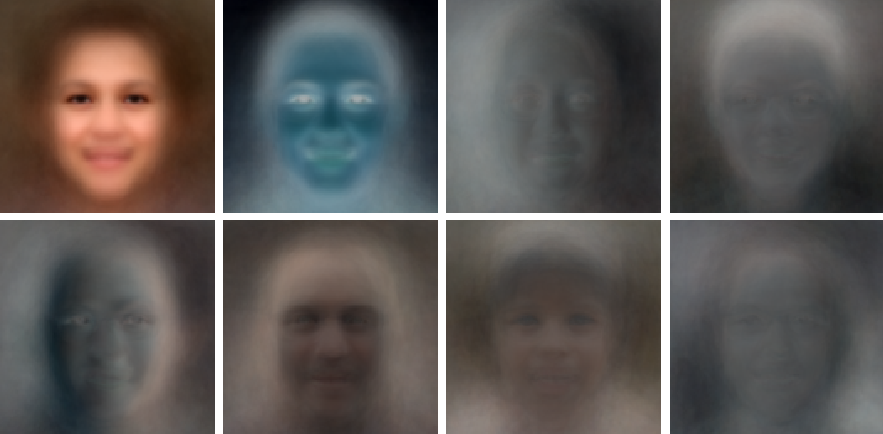
\includegraphics[height=3.2cm]{fig/PCA/pca}
     \caption{The first 8 eigenfaces from the FFHQ dataset.}
    \label{eigenfacehere}
    \end{subfigure}
    ~
    \begin{subfigure}[b]{0.4\textwidth}
        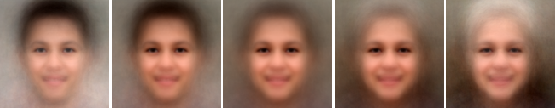
\includegraphics[height=1cm]{fig/PCA/pca3}
        
\includegraphics[height=1cm]{fig/PCA/pca4}
         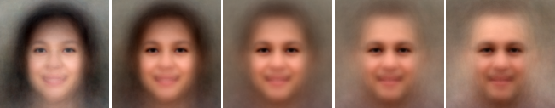
\includegraphics[height=1cm]{fig/PCA/pca5}
         \caption{Mean face shifted by the 4-6th eigenface.}
         \label{components}
    \end{subfigure}
     \caption{ In Figure. \ref{eigenfacehere} we see the eigenfaces of the FFHQ dataset while in Figure. \ref{components} we see the mean face edited by by adding or subtracting the 4-6th eigenface from the mean face according to eq.\ref{eigenface-interpolate}.}
\end{figure}
Although Principal Component Analysis enables us to generate new faces and manipulate different aspects of the synthesized faces the results are still blurry, and nowhere near as photo realistic as the faces we will be able to generate with a pretrained Generative Adversarial Network in Section \ref{stylegan}.

\subsection{VAE}
To train a Variational Autoencoder we use a modified version of the VAE implementation from the keras documentation \footnote{ Available here: \url{https://keras.io/examples/variational_autoencoder/}} which is a keras the implementation from the original VAE from \cite{vae1}. In the implementation the encoder and decoder are both modeled by multilayer perceptrons. We see a latent space dimension of 100 which is the same as for the DCGAN model which we present in the next subsection.

In Figure \ref{vaeresults} we see the result of training the VAE for 4000 epochs on a black and white version of the datasets. We choose to train for 4000 epochs as this is about the maximum durations which was possible to train in Google Colab before the runtime was reset. The training time for the FFHQ dataset was about 7-8 hours. We make the Jupyter notebook which generate these images available with this project.\footnote{Available here: \url{ https://github.com/renhaa/faces/blob/master/VAE.ipynb}}

\begin{figure}[h!]
\centering
\begin{subfigure}[b]{0.45\textwidth}
     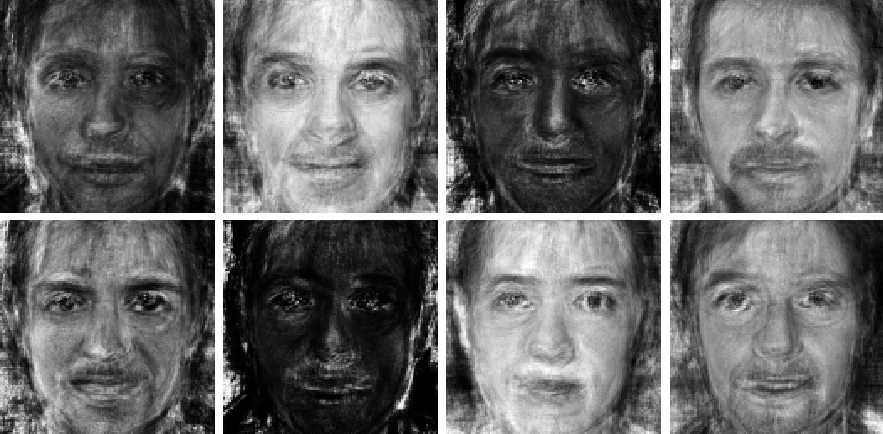
\includegraphics[width=\textwidth]{fig/vae/caltech_epoch4000}
    \caption{caltech}
\end{subfigure}
    ~
\begin{subfigure}[b]{0.45\textwidth}
     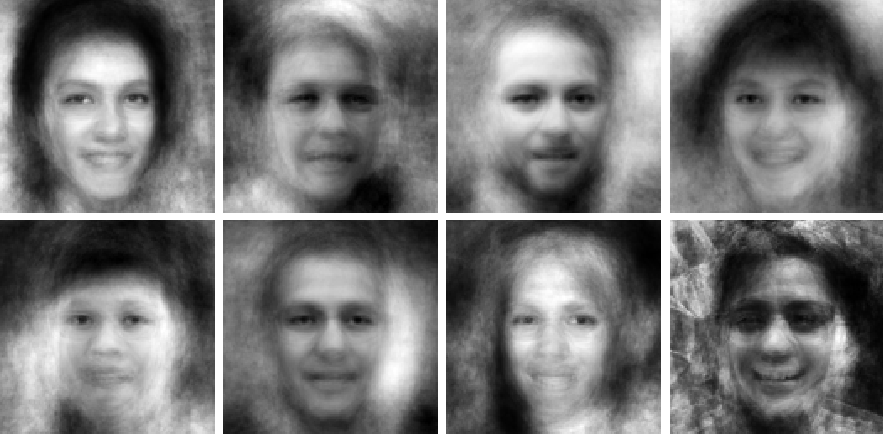
\includegraphics[width=\textwidth]{fig/vae/ffhq_epoch4000}
    \caption{ffhq}
\end{subfigure}
\caption{Samples from Variational Autoencoder during training on a black and white version of the Caltech and FFHQ dataset}
\label{vaeresults}
\end{figure}

Larger figures with samples drawn during training can be seen in Figure \ref{vaq-bwffhq-samples} and Figure \ref{vaq-bwcaltech-samples}.

We also tried to train the VAE on color images but the results were unstable. The images during training can be seen in Figure \ref{vaq-ffhq-samples}. As can bee seen in the figure it seems that the model was improving at least until epoch 2000. But then at epoch 4000 the network suddenly did not improve anymore and there was little variation in the generated samples. This problem also happened for the Caltech dataset.



\subsection{DCGAN}
In this section we will present our results with training a Deep Convolutional Generative Adversarial Network (DCGAN). \footnote{Concretely we use modified version of from \url{https://github.com/eriklindernoren/Keras-GAN/blob/master/dcgan/dcgan.py}} \footnote{The nodebook generating the results presented here can be found at: \url{https://github.com/renhaa/faces/blob/master/DCGAN.ipynb}}

The models uses four convolutional layers in with the generator and discriminator and the implementation follows the guidelines presented in \cite{dcgan} where we use strided convolutions, batch normalization and Leaky ReLU in the discriminator while the generator uses normal ReLU in all hidden layers exept the last where we use the hyperbolic tangent.In figure \ref{dcgan-results} we see the results from training a DCGAN the FFHQ and Caltech datasets for 10000 epochs. The training time was about 9-10 hours using Google Colab.

\begin{figure}[h!]
    \centering
    \begin{subfigure}[b]{0.45\textwidth}
        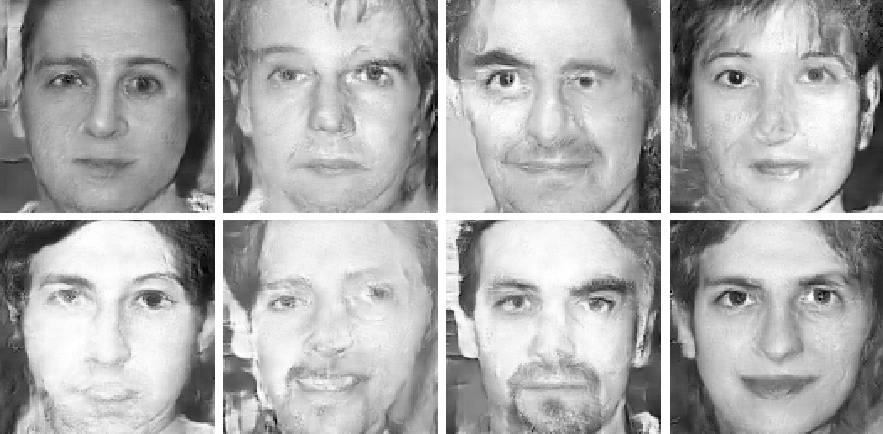
\includegraphics[width=\textwidth]{fig/dcgan/caltech/epoch10000}
        \caption{Caltech dataset B/W}
        \label{dcgan-caltech}
    \end{subfigure}
    ~
    \begin{subfigure}[b]{0.45\textwidth}
        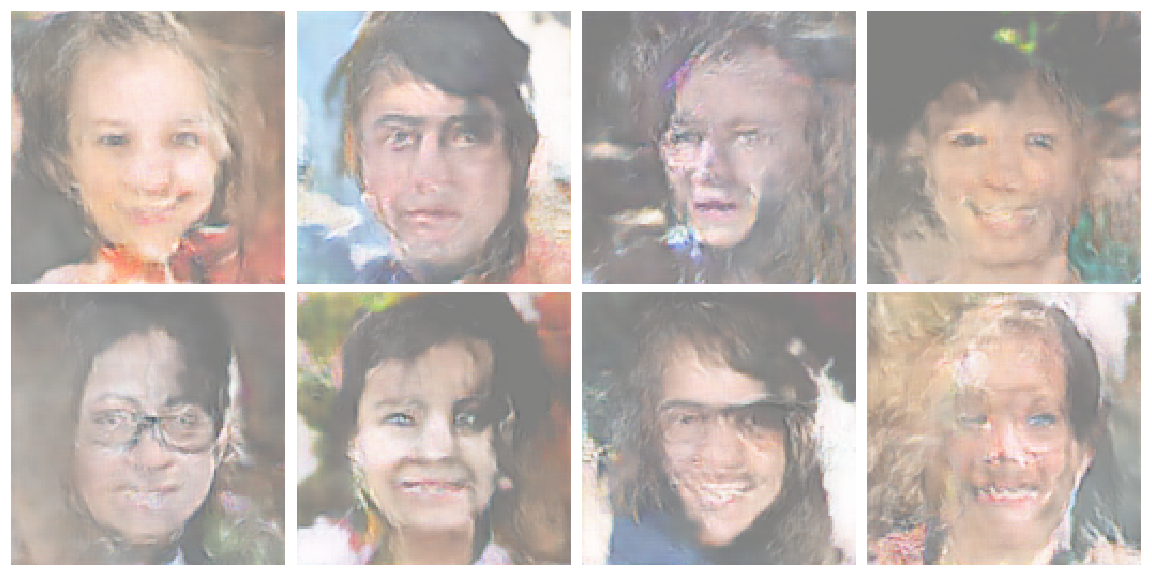
\includegraphics[width=\textwidth]{fig/dcgan/ffhq/epoch10000}
        \caption{FFHQ dataset}
        \label{dcgan-ffhq}
    \end{subfigure}
    \caption{The results from training the DCGAN for 10000 epochs on the FFHQ and Caltech datasets respectively.}
    \label{dcgan-results}
\end{figure}

We see that this model is able to produce relatively decent images on the black and white version of the Caltech dataset (Figure \ref{dcgan-caltech}). Sometimes we generate an image which could be mistaken for being real. Upon further inspection however, we note that the generated images are always somewhat similar to one of the 27 persons in the dataset. Thus it seem that we are able to create better quality images but with lower variation using the Caltech dataset compared to the FFHQ dataset. We argue that the generated images produced here by the DCGAN by training on the Caltech dataset are of better quality and than the corresponding images synthesized by the Variational Autoencoder from the previous subsection.

The generated images by training the DCGAN on the FFHQ are however, as we see in Figure \ref{dcgan-ffhq}, nowhere near photorealism, training for longer would almost certainly improve the results. 


\section{Exploring the latent space of StyleGAN}
\label{stylegan}
In this section we will explore  very regent advances in face synthesis\footnote{} in use a pretrained

\subsection{StyleGAN}

We can download the weigths of a pre-trained stylegan trained by Nvidia\footnote{\url{https://github.com/NVlabs/stylegan.git}}\cite{stylegan}
The model is trained on the full size and resolution version of the FFHQ dataset.
With the trained generator we can draw sample $z$ from the normal distribution and generate faces $G(x)$ which are near impossible to humans to distinguish from real faces.

In Figure \ref{StyleGAN-examples} we see eight such samples. We can create as many photo realistic faces, of people who have existed, as we want.
\begin{figure}[h!]
  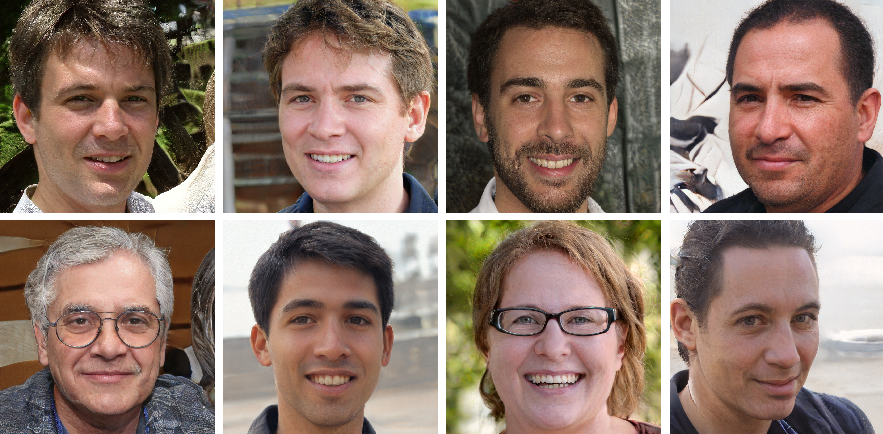
\includegraphics[width=\textwidth]{fig/stylegan/randomsamples}
  \caption{Random samples from the pretrained StyleGAN}
  \label{StyleGAN-examples}
\end{figure}




\subsubsection{Finding the latent space representation of an arbitrary query image.}
Now the pretrained StyleGAN does not contain an encoder network. Therefore there is no way to find a latent space representation of a arbitrary input image.
There is, however a a least two different ways of tackling this problem.
%
% One is the optimization-based
% approach, which directly optimizes the latent code with fixed generator to minimize the pixel-wise reconstruction error [22]. The other is the encoder-based, where an independent encoder network is trained to learn the inverse mapping [37].
\cite{interfacegan}
The paper \textit{Image2StyleGAN: How to Embed Images Into the StyleGAN Latent Space?}\cite{Image2StyleGAN} explicitly investigates this problem.


Here we use the first approach where hold the pretrained generator fixed and then optimize the latent vector to give the desired output image. But instead of calculating the loss directly on the pixel-wise reconstruction error. \footnote{Here we use the codebase provided at: \url{https://github.com/Puzer/stylegan-encoder}}

Here we use the same approach as in \cite{styletransfer} where

We use a pre-trained VGG16 network for transforming a query image and the generated image from the latent vector into a high dimensional feature space. The loss is them calculated as a difference between the two feature vectors in the VGG16 feature space.

\begin{figure}
    \centering
    \begin{subfigure}[b]{\textwidth}
        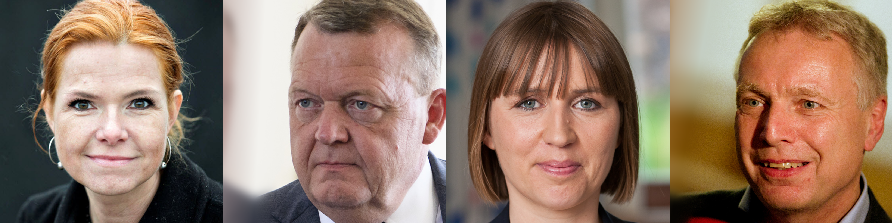
\includegraphics[width=\textwidth]{fig/stylegan/originals}
        \caption{Original images.}
    \end{subfigure}
    \begin{subfigure}[b]{\textwidth}
        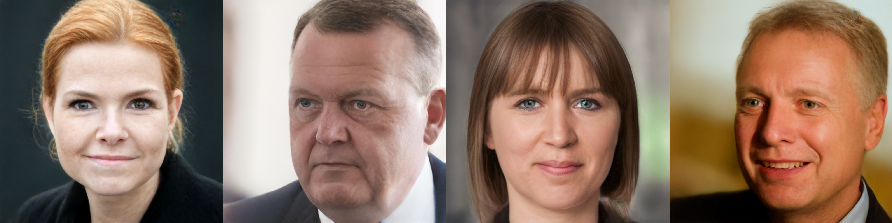
\includegraphics[width=\textwidth]{fig/stylegan/reconstructions}
        \caption{Reconstructed images.}
    \end{subfigure}
    \caption{Comparison of original query images and their reconstruction in the StyleGAN network}
    \label{stylegan-reconstruction}
\end{figure}

We can to a linear interpolation between two latent vectors $z_1$ and $z_2$ simply by
\begin{align}
  z = \alpha z_2 + (1-\alpha)z_1
\end{align}
for $0 \leq \alpha \leq 1$. This linear interpolation results in images that smoothly transitions between faces generated by $z_1$ and $z_2$ respectively. In Figure \ref{StyleGAN-interpolation} we see the result of doing a linear interpolation between the latent representations of the two last danish prime ministers.

\begin{figure}
  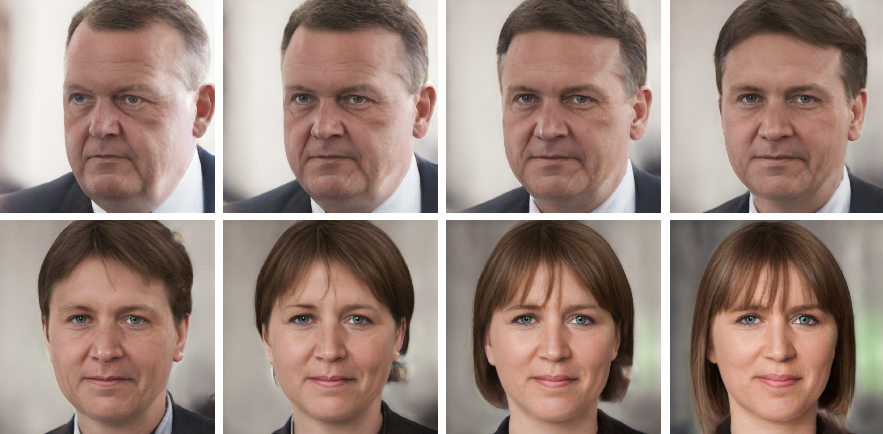
\includegraphics[width=\textwidth]{fig/stylegan/interpolation}
  \caption{Interpolation between two StyleGAN images}
  \label{StyleGAN-interpolation}
\end{figure}


% Optimization is performed only for latent representation which we want to obtain.

% Upon completion of optimization you are able to transform your latent vector as you wish. For example you can find a "smiling direction" in your latent space, move your latent vector in this direction and transform it back to image using the generator.

%
% \begin{figure}[htb]
%     \centering
%     \begin{subfigure}[b]{\textwidth}
%         \centering
%         
\includegraphics[width=0.3\linewidth]{fig/query_images/trump}%
%         \hfill
%         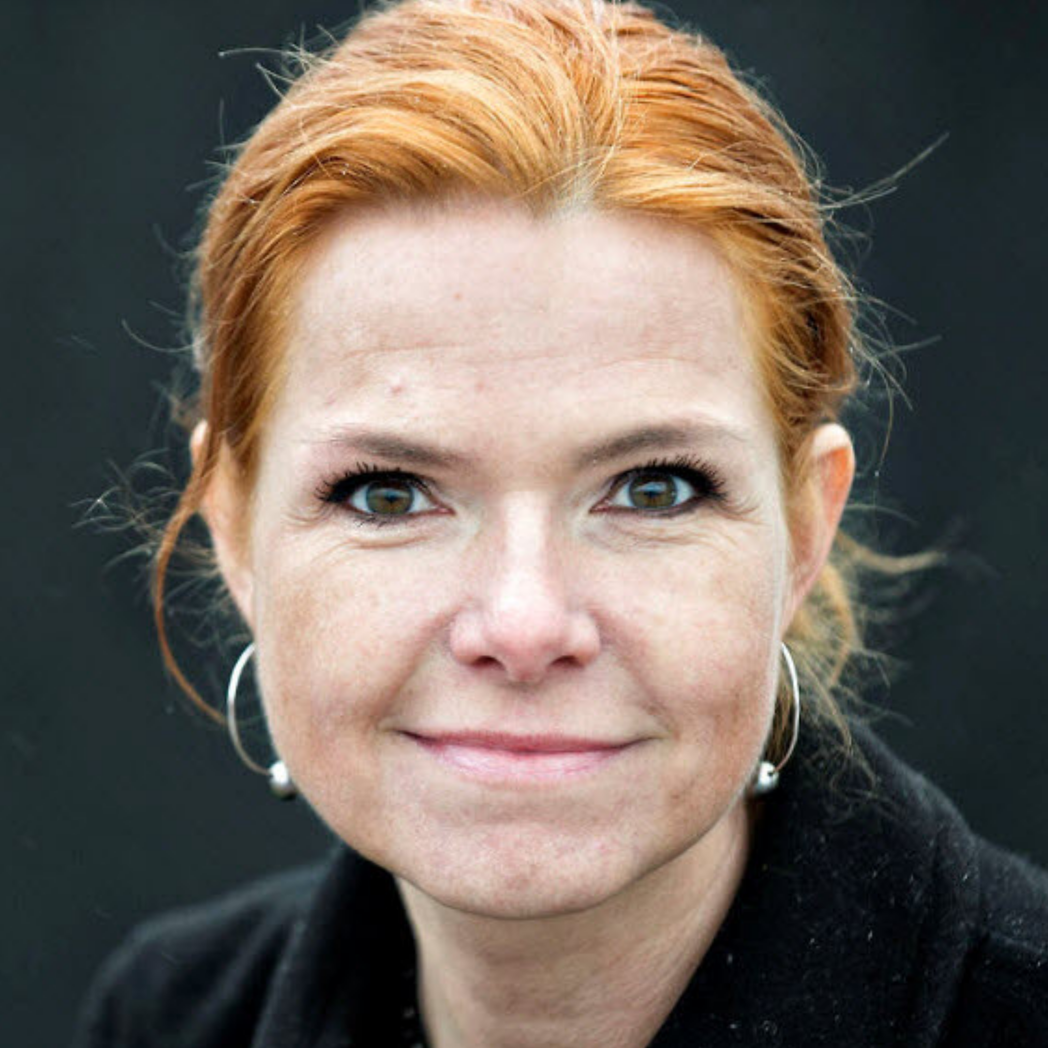
\includegraphics[width=0.3\linewidth]{fig/query_images/inger}
%         \hfill
%         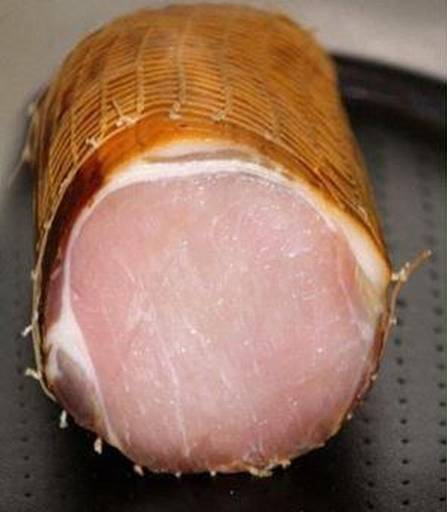
\includegraphics[width=0.3\linewidth]{fig/query_images/skinke}
%         \caption{Original Query Images}
%     \end{subfigure}
%     \vskip\baselineskip
%     \begin{subfigure}[b]{\textwidth}
%         \centering
%         
\includegraphics[width=0.3\linewidth]{fig/query_images_reconstucted/trump}%
%         \hfill
%         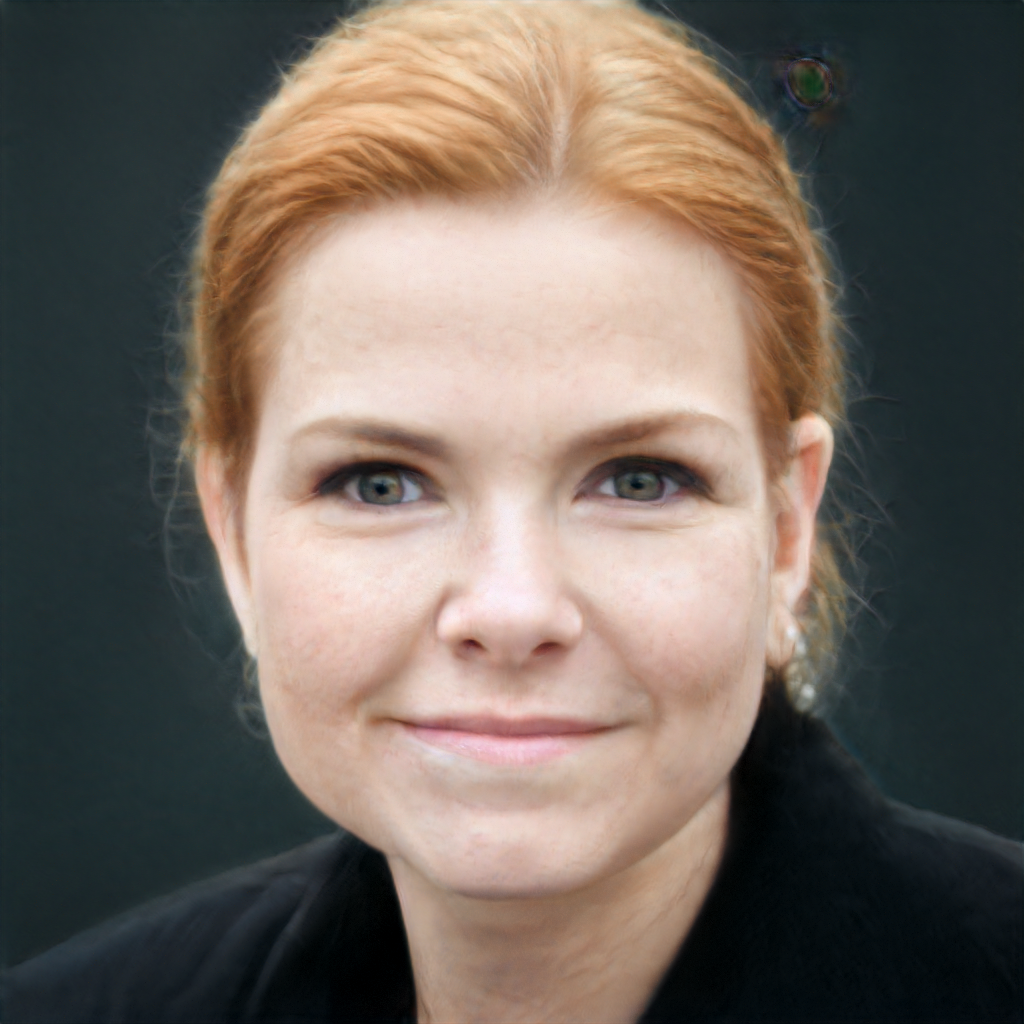
\includegraphics[width=0.3\linewidth]{fig/query_images_reconstucted/inger}
%         \hfill
%         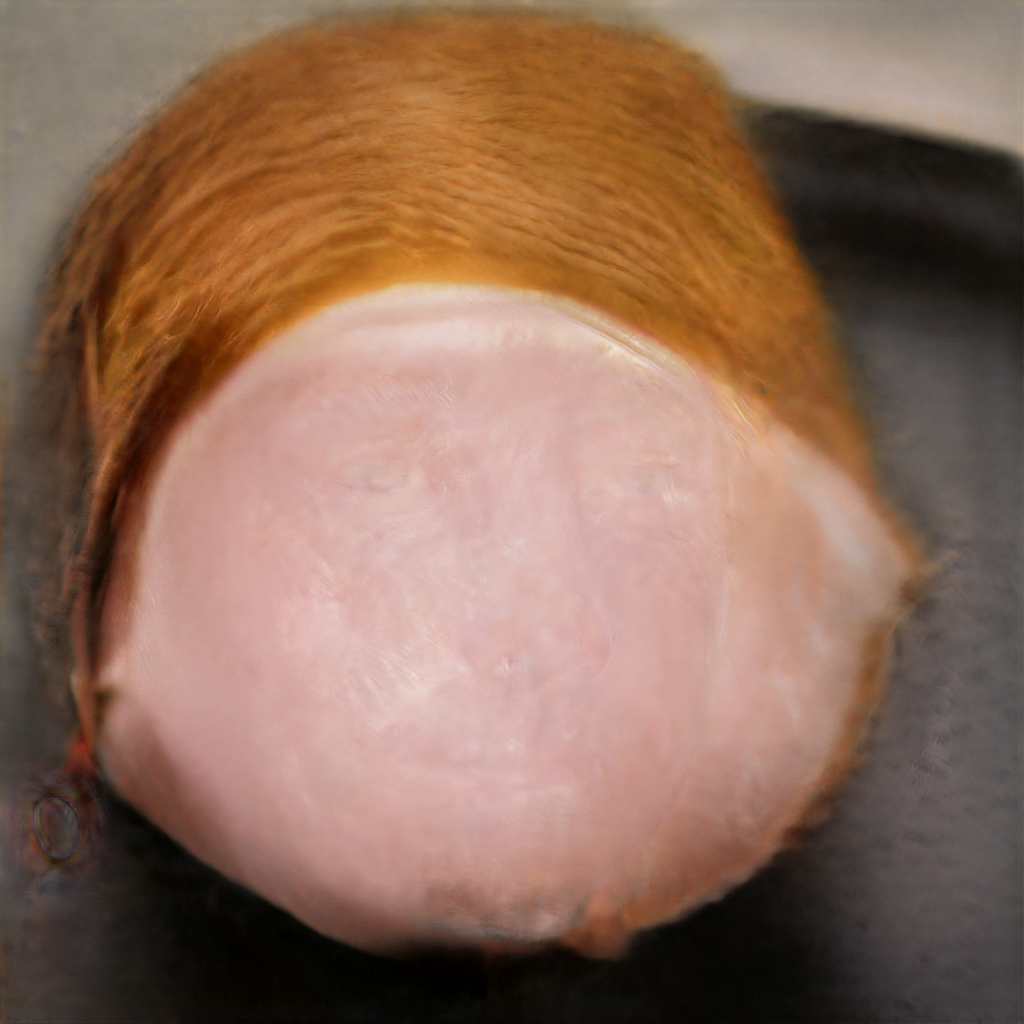
\includegraphics[width=0.3\linewidth]{fig/query_images_reconstucted/skinke}
%         \caption{Reconstructed images from StyleGAN latent space}
%     \end{subfigure}
%     \caption{Latent space representation of arbitrary query images }
% \end{figure}

% \begin{figure}
%     \centering
%     \begin{subfigure}[b]{0.45\textwidth}
%         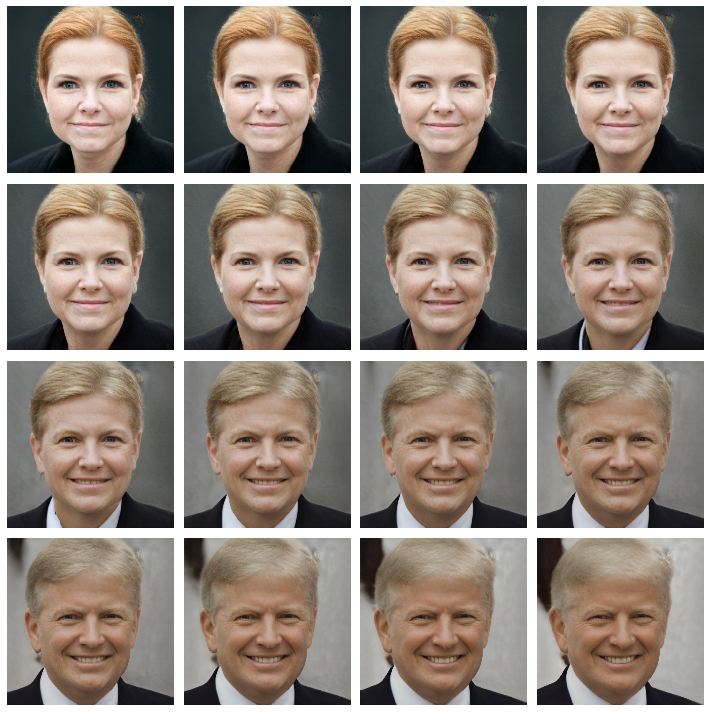
\includegraphics[width=\textwidth]{fig/ingertrump}
%         \caption{Inger Støjberg to Donald Trump}
%     \end{subfigure}
%     ~
%     \begin{subfigure}[b]{0.45\textwidth}
%         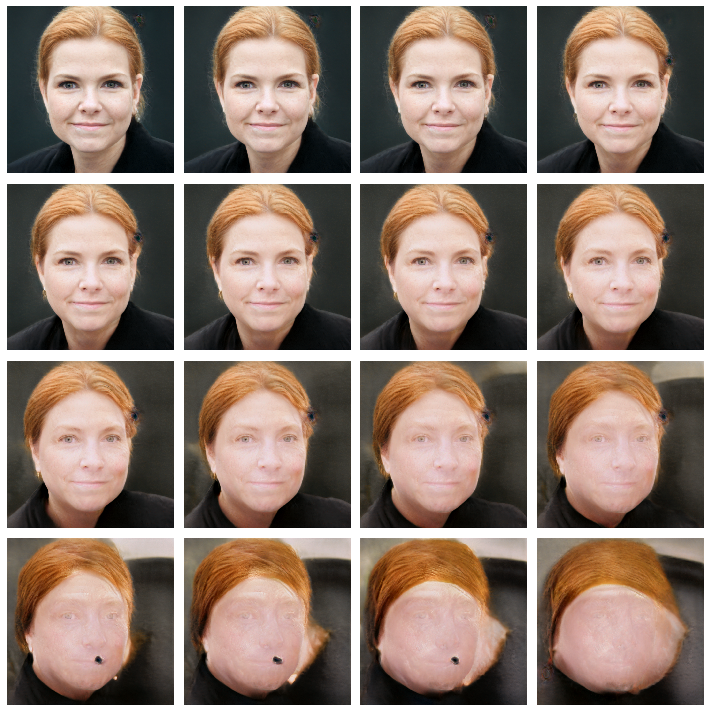
\includegraphics[width=\textwidth]{fig/ingerham}
%         \caption{Inger Støjberg to Ham}
%     \end{subfigure}
%     \caption{Interpolations between query images in the StyleGAN latent space.}
% \end{figure}

\subsubsection{Semantic face editing.}

In Figure \ref{faceedit} we see the results from doing semantic face editing of the reconstructed images from
\ref{stylegan-reconstruction}.

\begin{figure}[h!]
    \centering
    \begin{subfigure}[b]{0.24\textwidth}
        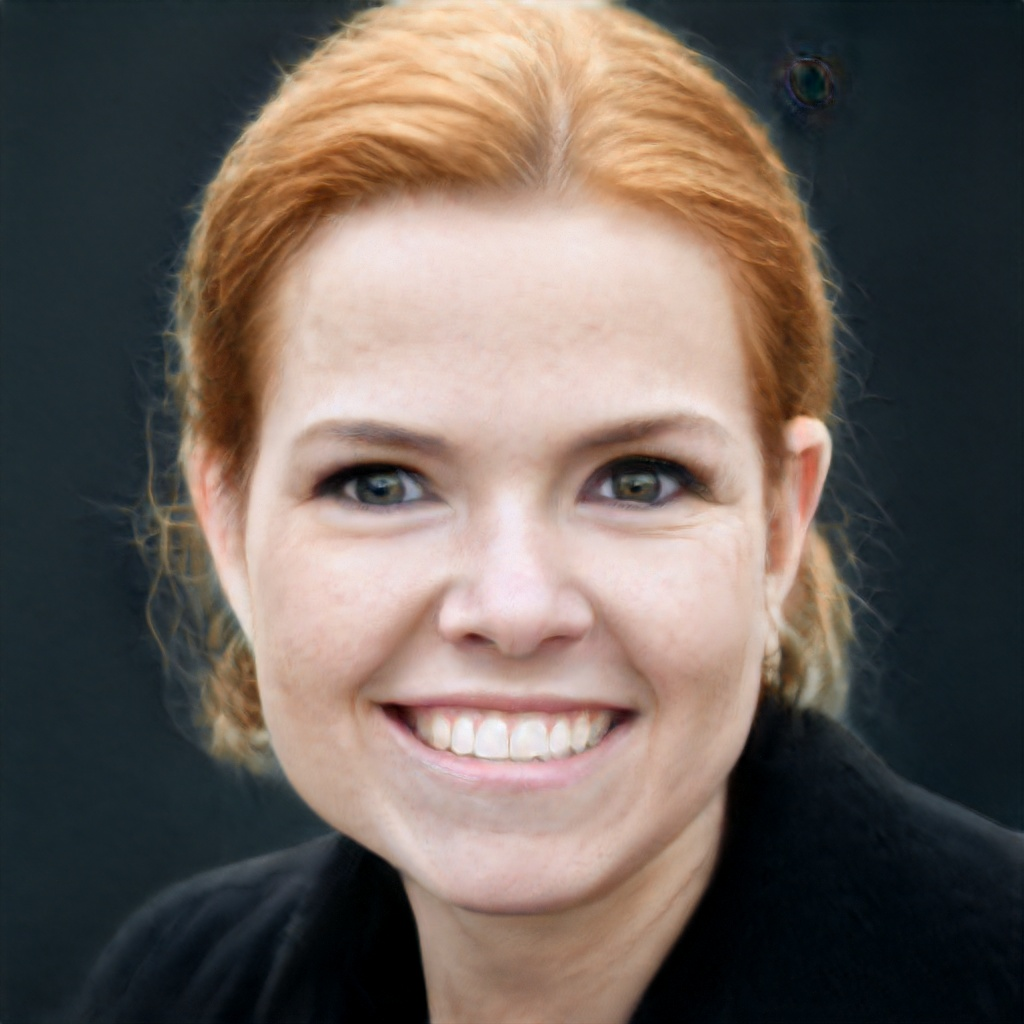
\includegraphics[width=\textwidth]{fig/stylegan/faceedit/inger-smile}

    \end{subfigure}
    \begin{subfigure}[b]{0.24\textwidth}
        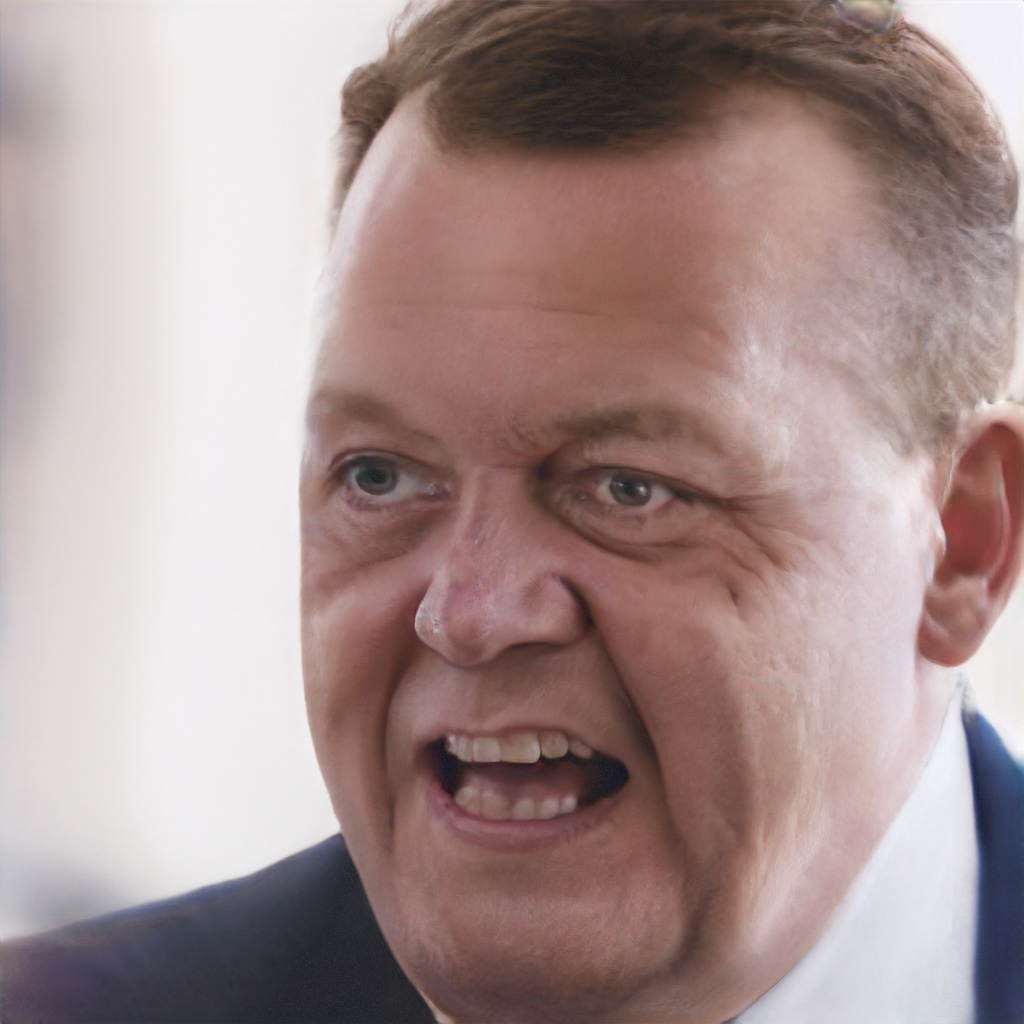
\includegraphics[width=\textwidth]{fig/stylegan/faceedit/lars-smile}

    \end{subfigure}
    \begin{subfigure}[b]{0.24\textwidth}
        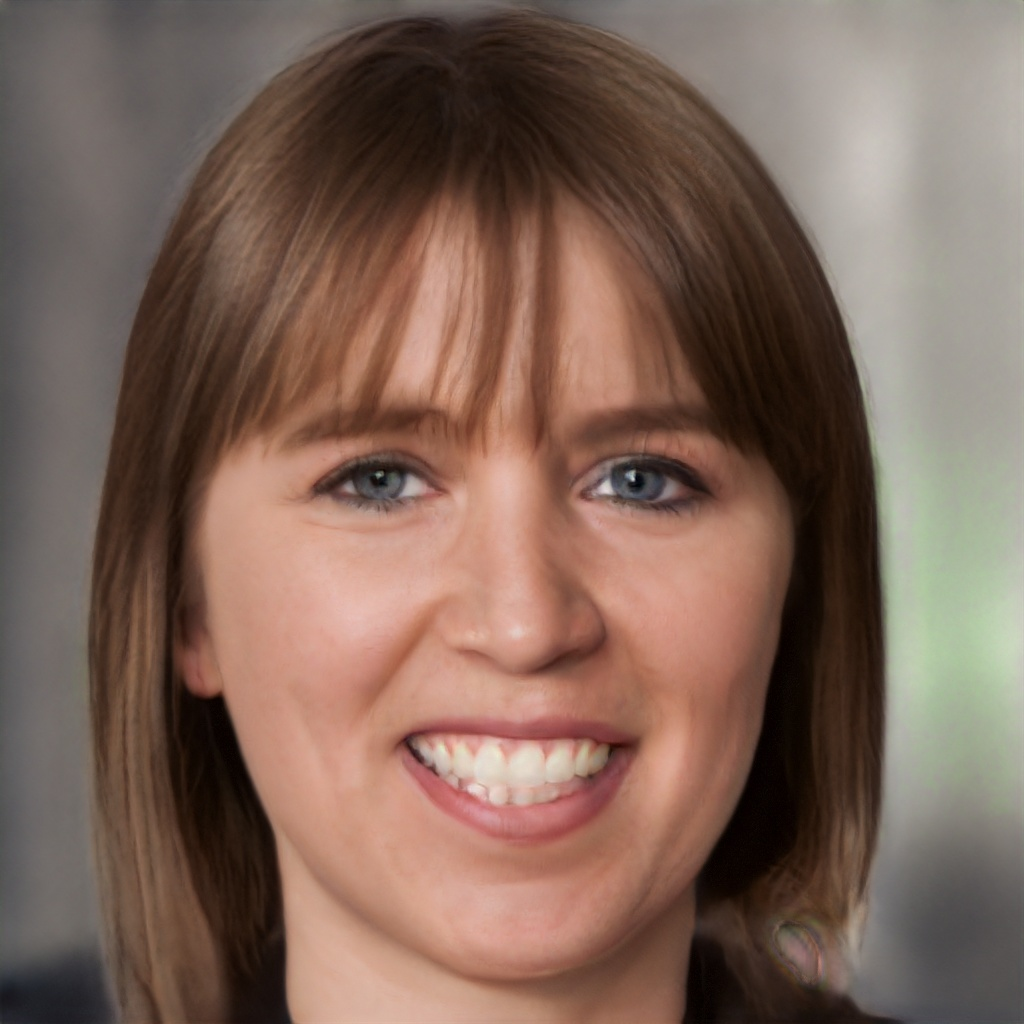
\includegraphics[width=\textwidth]{fig/stylegan/faceedit/mette-smile}

    \end{subfigure}
    \begin{subfigure}[b]{0.24\textwidth}
        
\includegraphics[width=\textwidth]{fig/stylegan/faceedit/uffe-smile}

    \end{subfigure}

    \begin{subfigure}[b]{0.24\textwidth}
        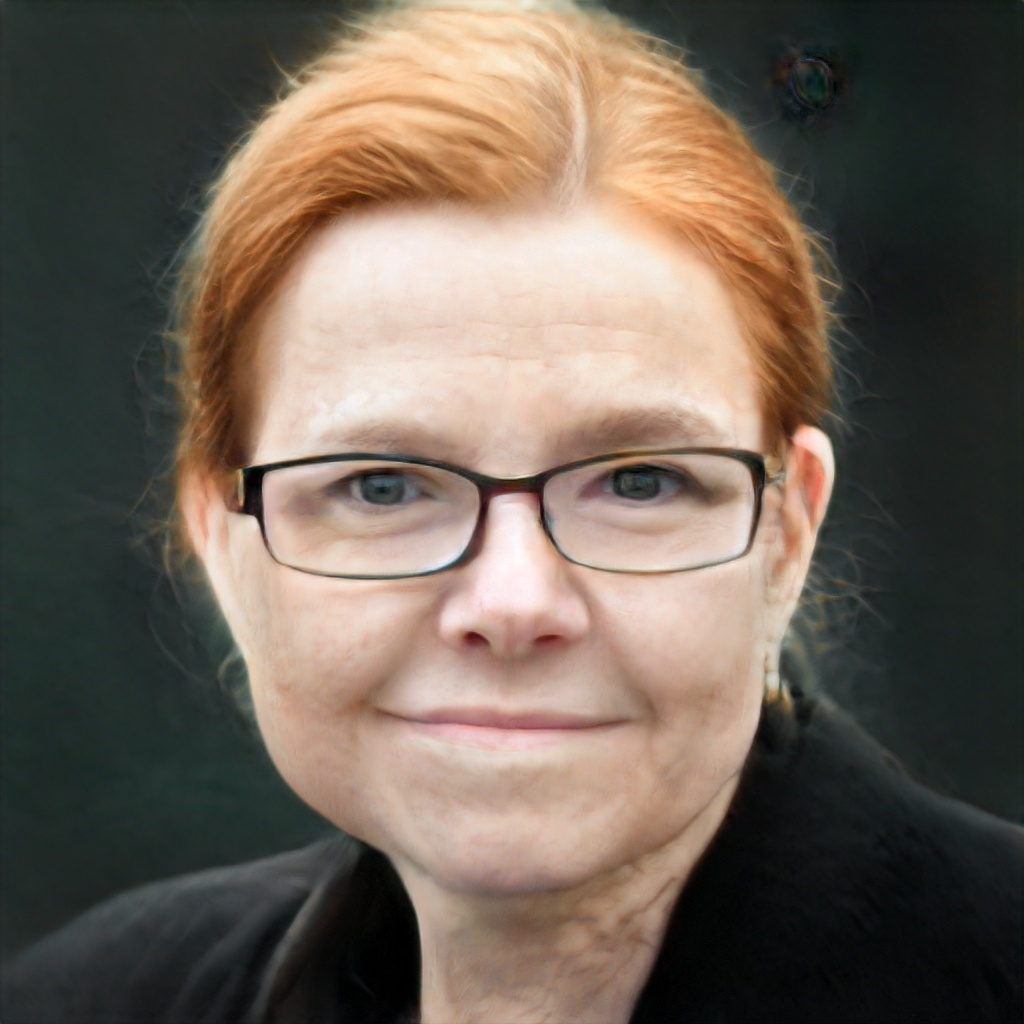
\includegraphics[width=\textwidth]{fig/stylegan/faceedit/inger-glasses}

    \end{subfigure}
    \begin{subfigure}[b]{0.24\textwidth}
        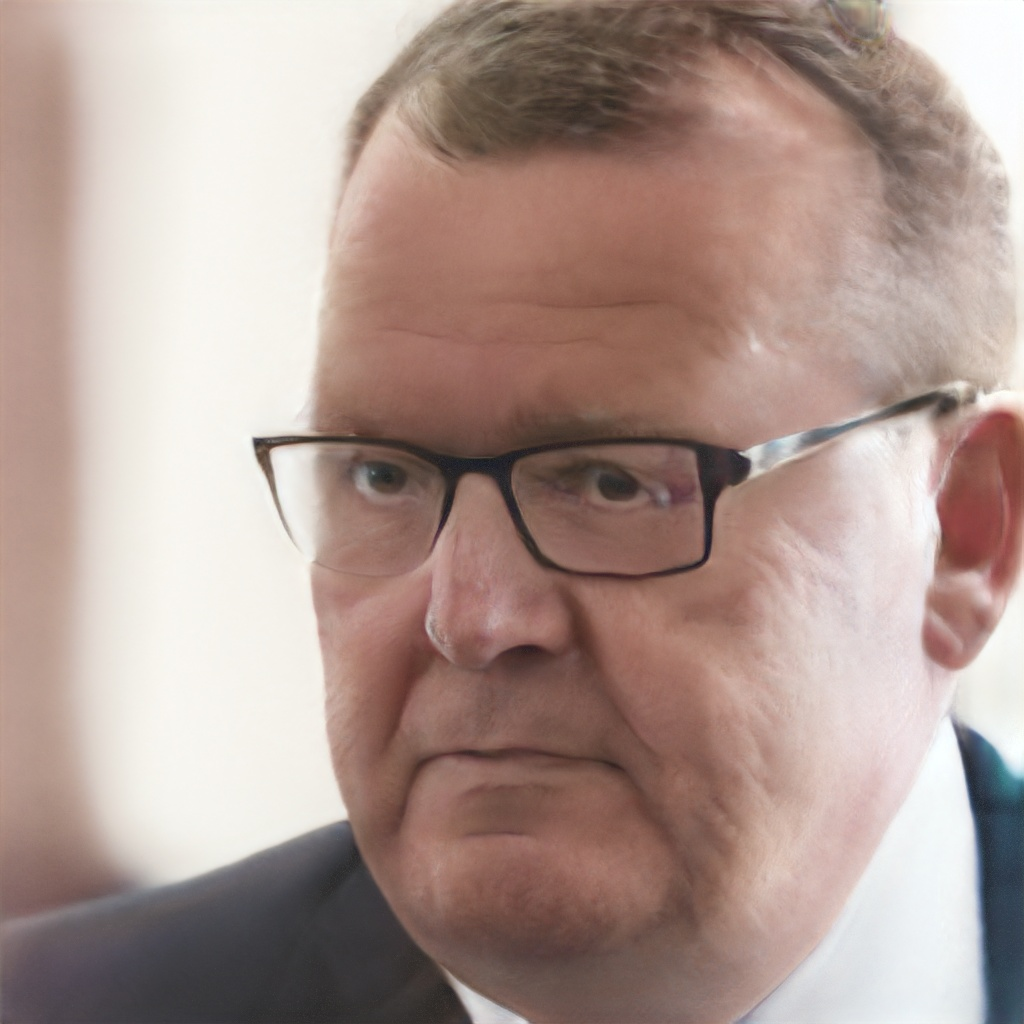
\includegraphics[width=\textwidth]{fig/stylegan/faceedit/lars-glasses}

    \end{subfigure}
    \begin{subfigure}[b]{0.24\textwidth}
        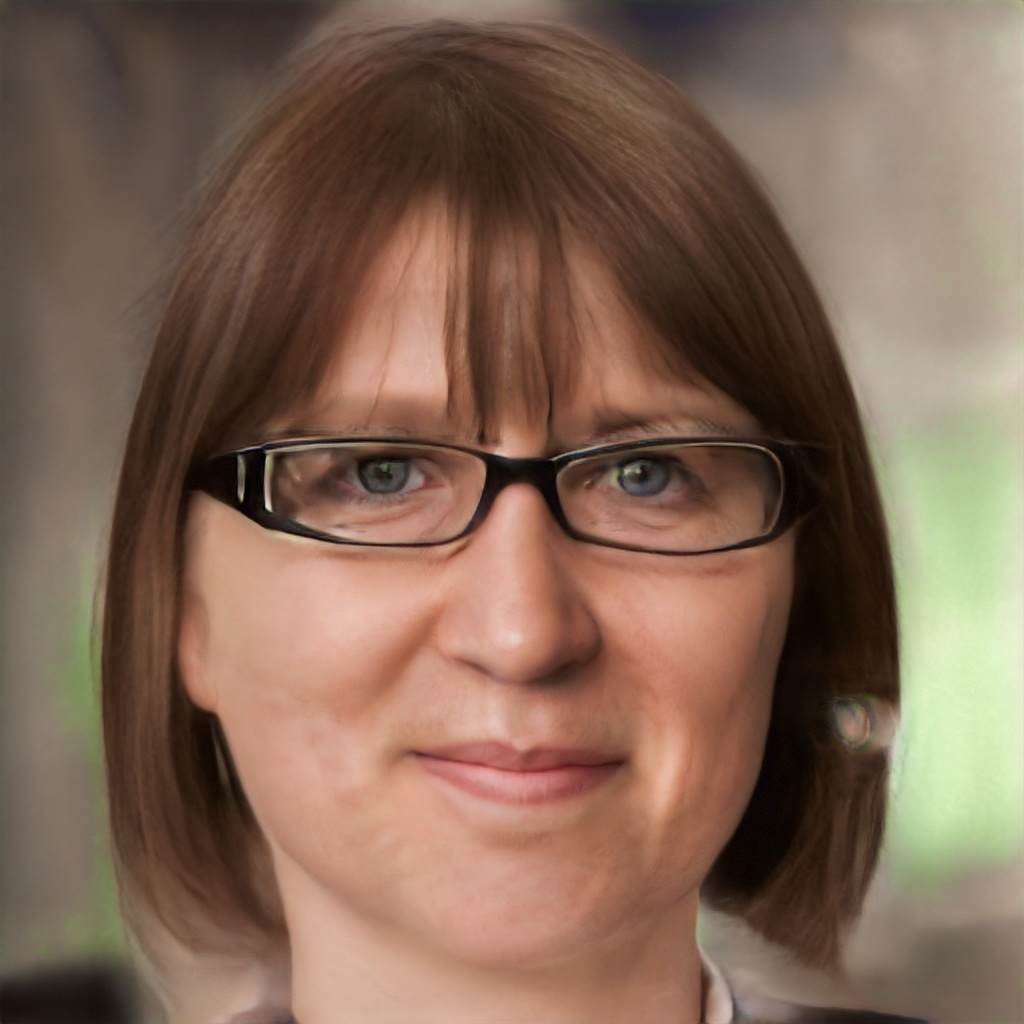
\includegraphics[width=\textwidth]{fig/stylegan/faceedit/mette-glasses}

    \end{subfigure}
    \begin{subfigure}[b]{0.24\textwidth}
        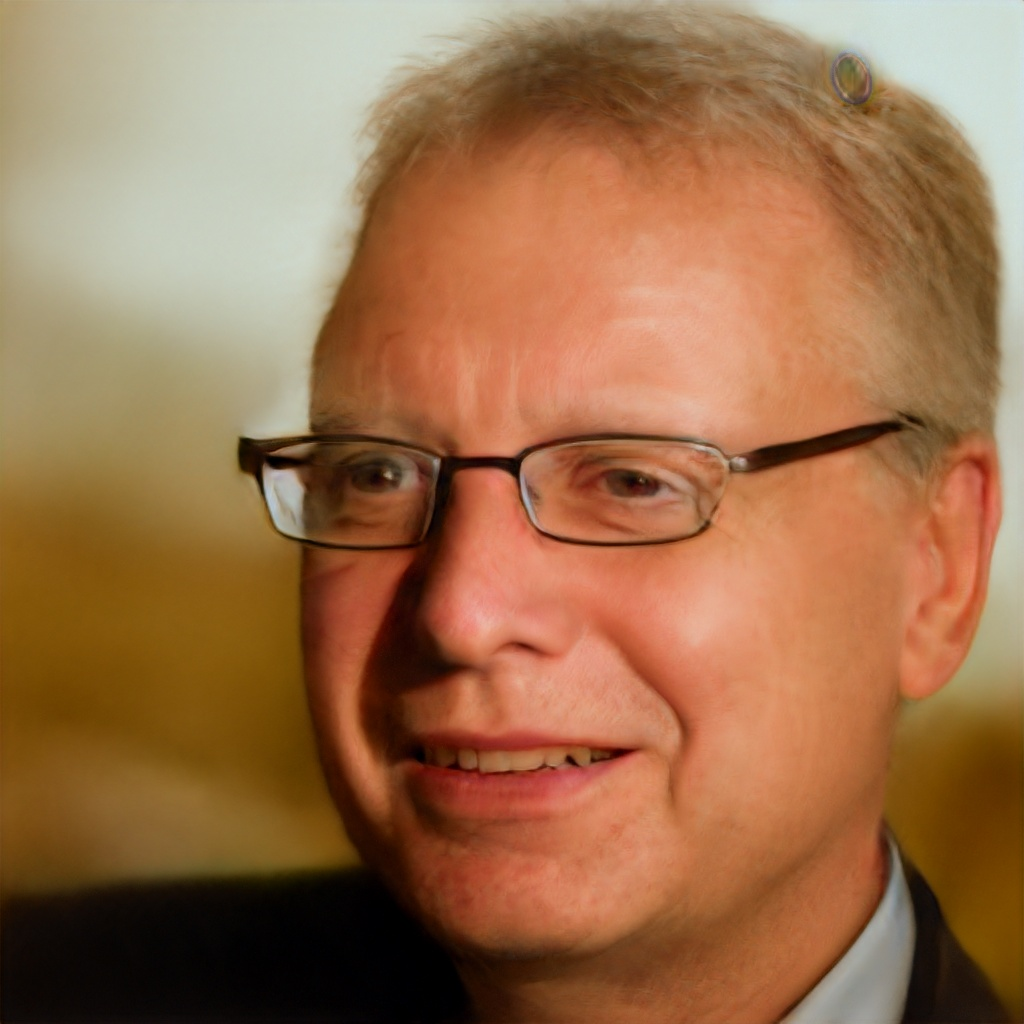
\includegraphics[width=\textwidth]{fig/stylegan/faceedit/uffe-glasses}

    \end{subfigure}

    \begin{subfigure}[b]{0.24\textwidth}
        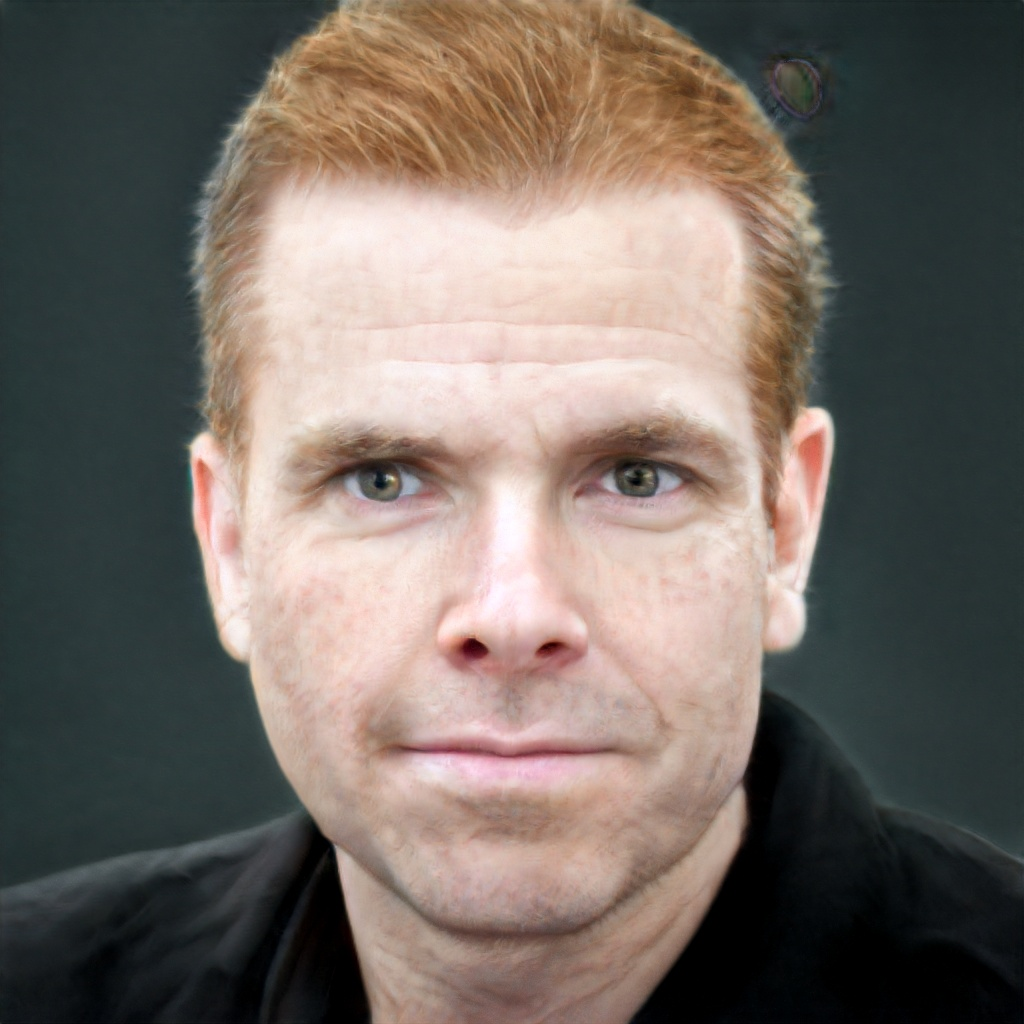
\includegraphics[width=\textwidth]{fig/stylegan/faceedit/inger-gender}

    \end{subfigure}
    \begin{subfigure}[b]{0.24\textwidth}
        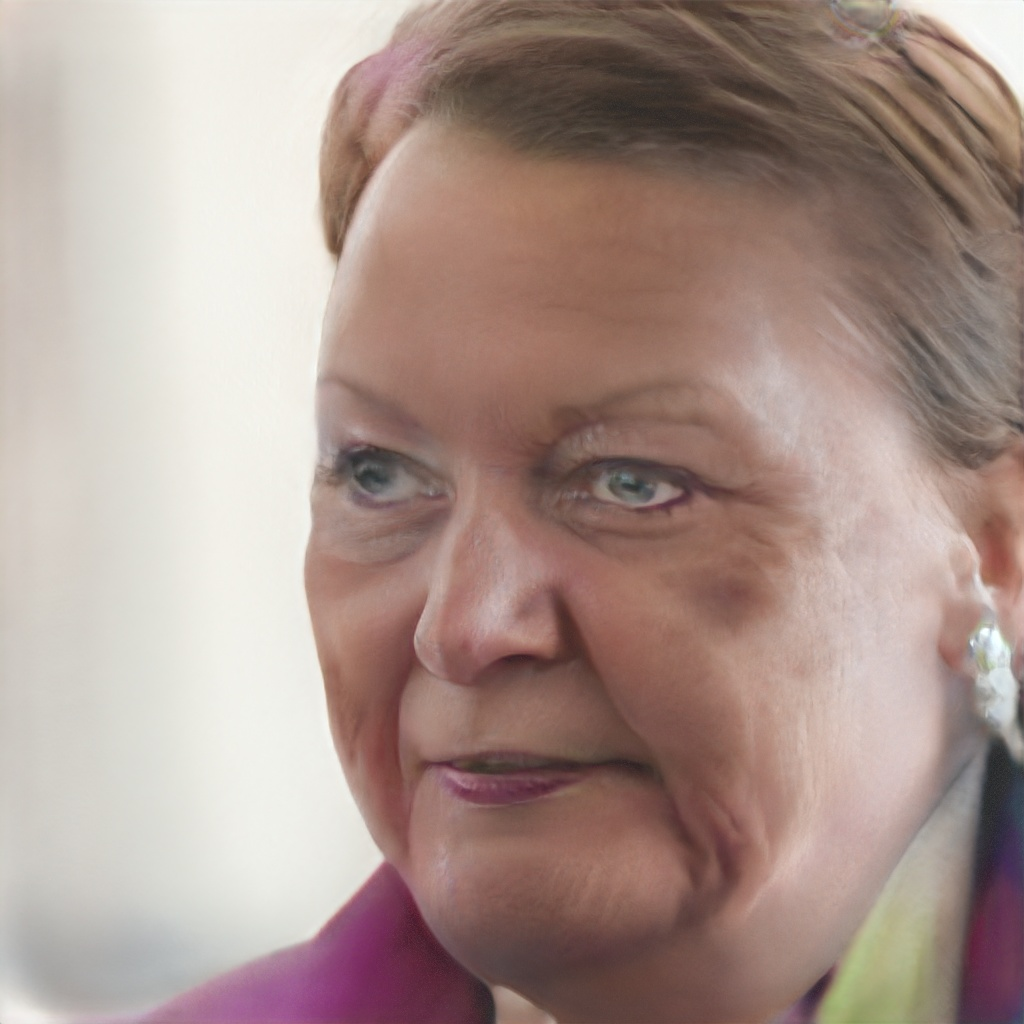
\includegraphics[width=\textwidth]{fig/stylegan/faceedit/lars-gender}

    \end{subfigure}
    \begin{subfigure}[b]{0.24\textwidth}
        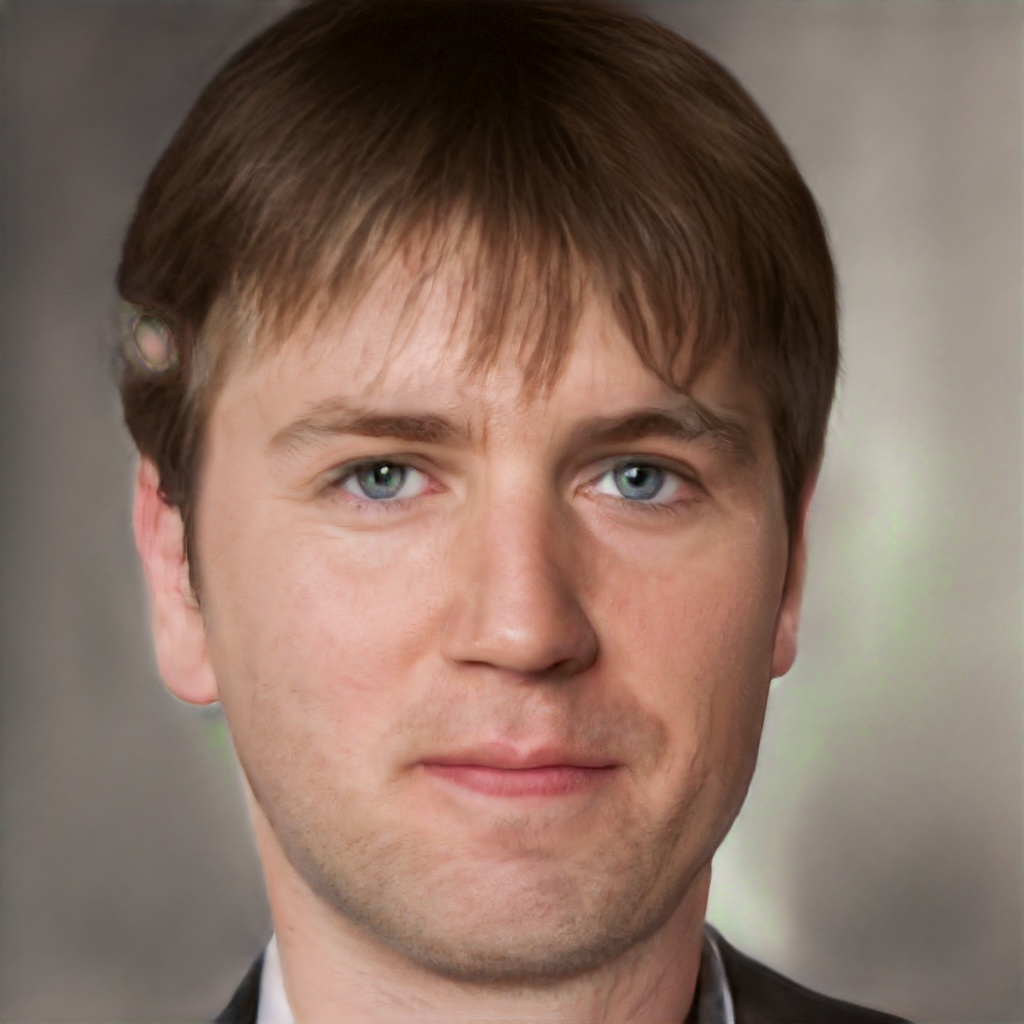
\includegraphics[width=\textwidth]{fig/stylegan/faceedit/mette-gender}

    \end{subfigure}
    \begin{subfigure}[b]{0.24\textwidth}
        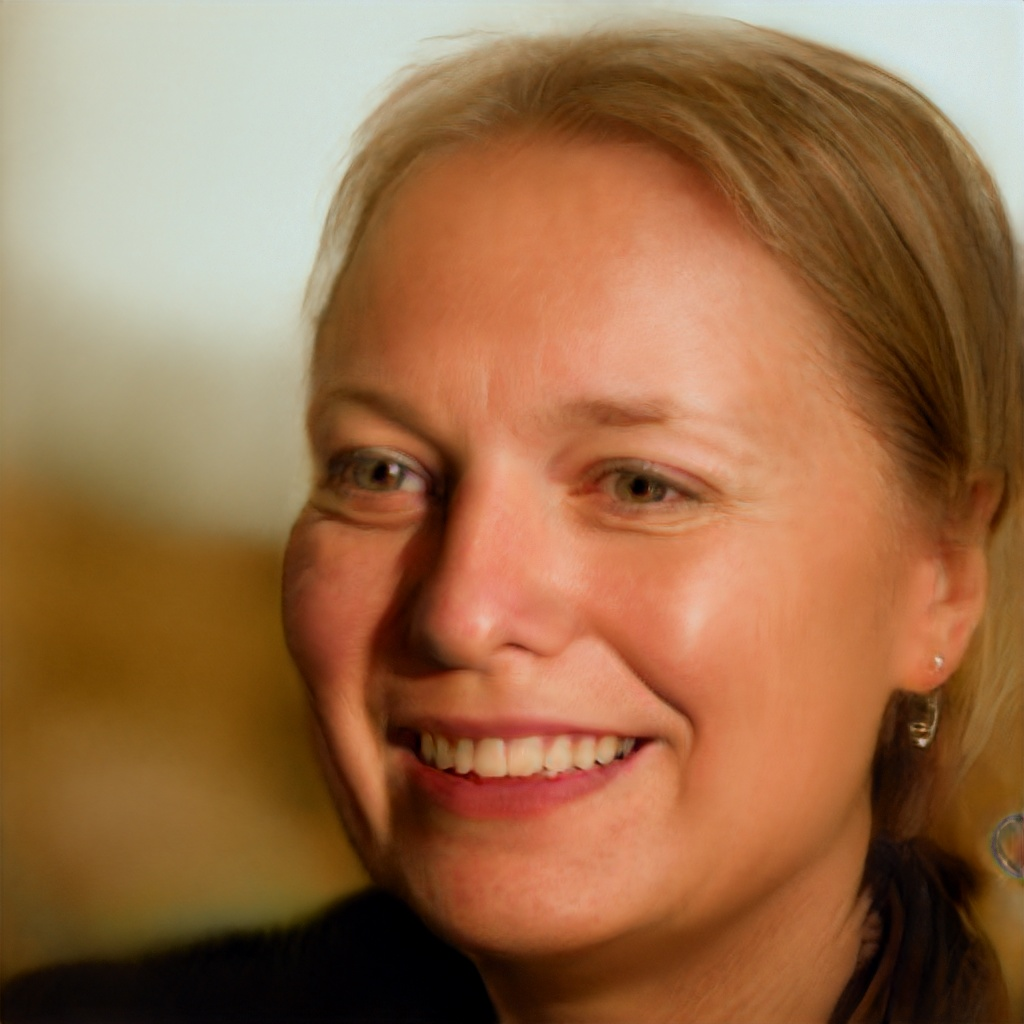
\includegraphics[width=\textwidth]{fig/stylegan/faceedit/uffe-gender}

    \end{subfigure}
    \caption{Semantic face editing.}
    \label{faceedit}
\end{figure}

\section{Conclusion}


\newpage
\bibliography{references}
\bibliographystyle{plain}
\newpage
\appendix
\counterwithin{figure}{section}

\section{Appendix}

\begin{figure}[h!]
  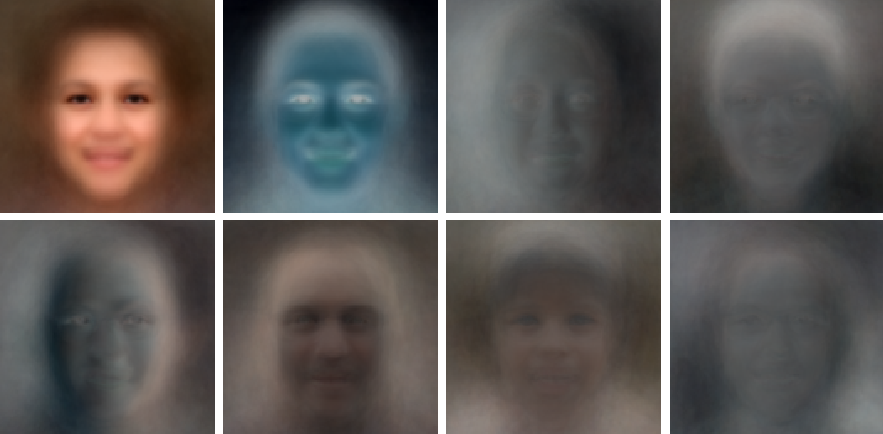
\includegraphics[width=\textwidth]{fig/PCA/pca}
  \caption{Eigenfaces of the FFHQ dataset.}
  \label{eigenface}
\end{figure}

\begin{figure} [h!]
    \centering
    \begin{subfigure}[b]{\textwidth}
        
\includegraphics[width=\textwidth]{fig/PCA/pca0}
   
    \end{subfigure}
    \begin{subfigure}[b]{\textwidth}
        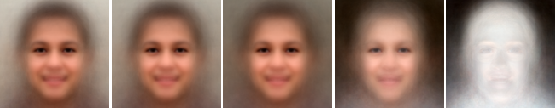
\includegraphics[width=\textwidth]{fig/PCA/pca1}
       
    \end{subfigure}
    \begin{subfigure}[b]{\textwidth}
        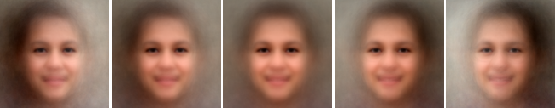
\includegraphics[width=\textwidth]{fig/PCA/pca2}
       
    \end{subfigure}
    \begin{subfigure}[b]{\textwidth}
        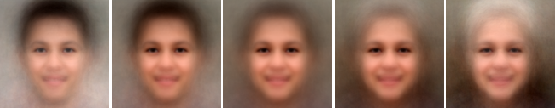
\includegraphics[width=\textwidth]{fig/PCA/pca3}
       
    \end{subfigure}
    \begin{subfigure}[b]{\textwidth}
        
\includegraphics[width=\textwidth]{fig/PCA/pca4}

    \end{subfigure}
    \begin{subfigure}[b]{\textwidth}
        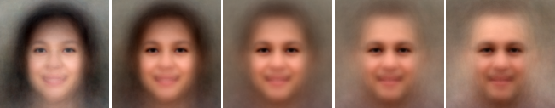
\includegraphics[width=\textwidth]{fig/PCA/pca5}

    \end{subfigure}
    \caption{Synthetic faces created by varying a single principal component to the mean face if the FFHQ dataset. The rows correspond to the principal components such that the first row is the first compoment and so on. }
    \label{pca-components}
\end{figure}

%% VAE
\begin{figure}[h!]
    \centering
    \begin{subfigure}[b]{0.45\textwidth}
        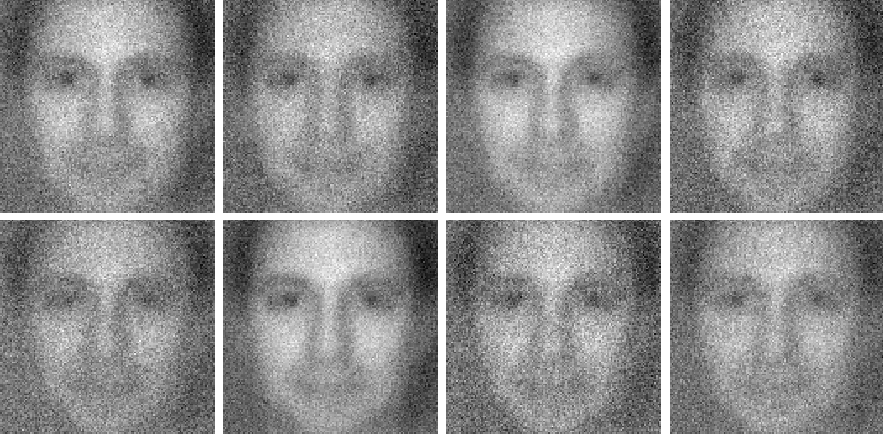
\includegraphics[width=\textwidth]{fig/vae/caltech_epoch50}
        \caption{Epoch 50}
    \end{subfigure}
    ~
    \begin{subfigure}[b]{0.45\textwidth}
         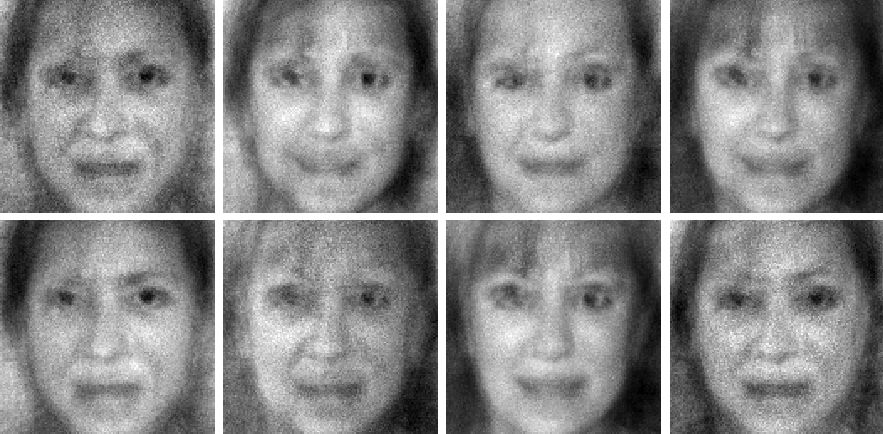
\includegraphics[width=\textwidth]{fig/vae/caltech_epoch400}
        \caption{Epoch 400}
    \end{subfigure}

    \begin{subfigure}[b]{0.45\textwidth}
         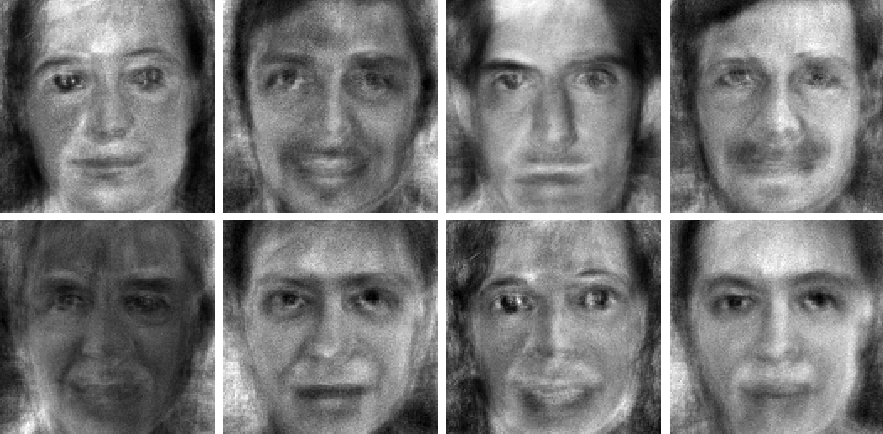
\includegraphics[width=\textwidth]{fig/vae/caltech_epoch1000}
        \caption{Epoch 1000}
    \end{subfigure}
    ~
    \begin{subfigure}[b]{0.45\textwidth}
         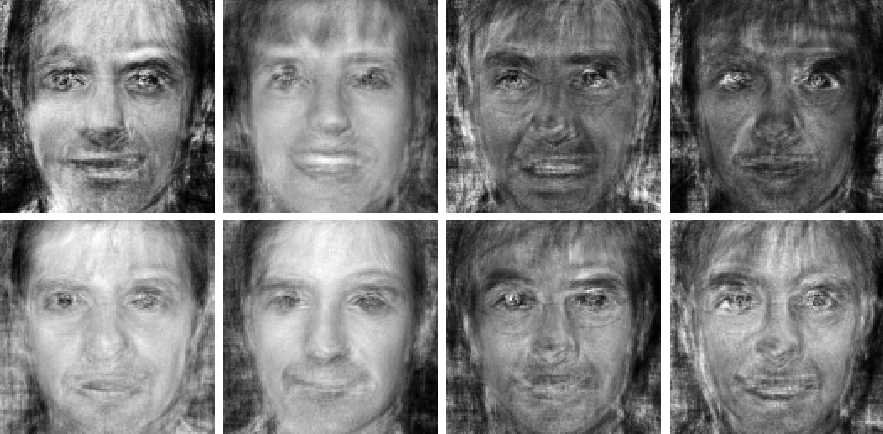
\includegraphics[width=\textwidth]{fig/vae/caltech_epoch2000}
        \caption{Epoch 2000}
    \end{subfigure}

    \begin{subfigure}[b]{\textwidth}
         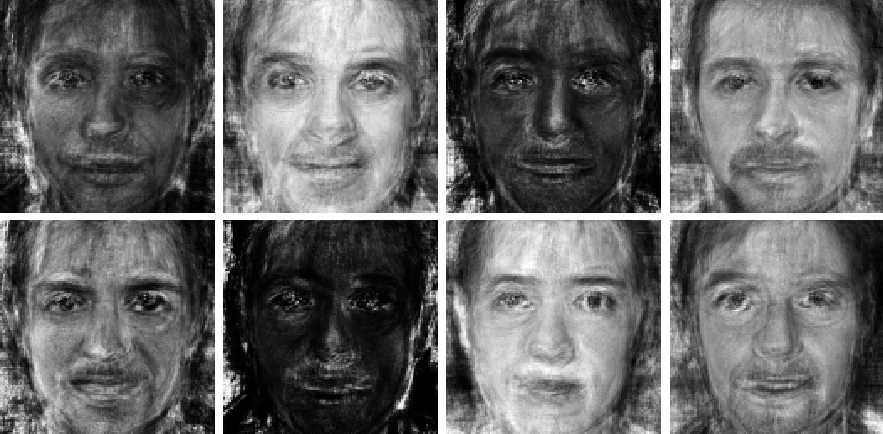
\includegraphics[width=\textwidth]{fig/vae/caltech_epoch4000}
        \caption{Epoch 4000}
    \end{subfigure}
    \caption{Samples from Variational Autoencoder  during training on a black and white version of the Caltech dataset}
    \label{vaq-bwcaltech-samples}
\end{figure}

\begin{figure}[h!]
    \centering
    \begin{subfigure}[b]{0.45\textwidth}
        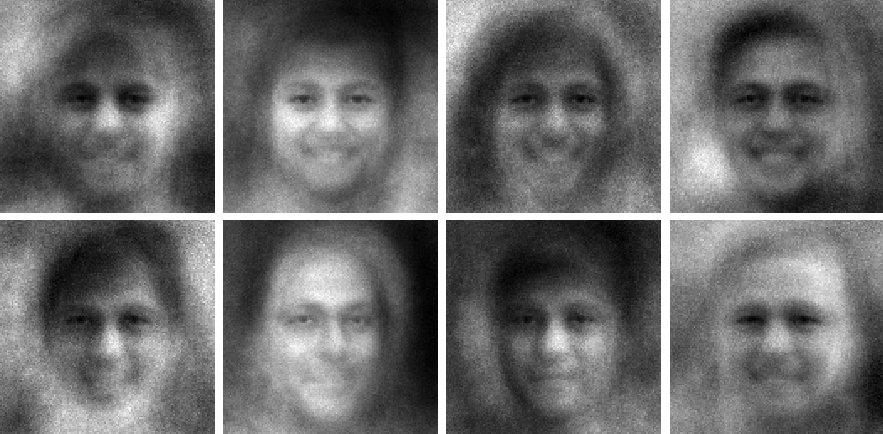
\includegraphics[width=\textwidth]{fig/vae/ffhq_epoch50}
        \caption{Epoch 50}
    \end{subfigure}
    ~
    \begin{subfigure}[b]{0.45\textwidth}
         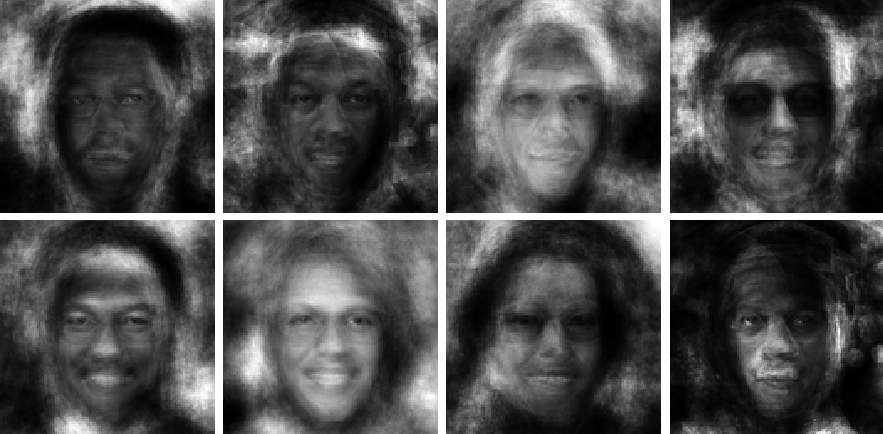
\includegraphics[width=\textwidth]{fig/vae/ffhq_epoch400}
        \caption{Epoch 400}
    \end{subfigure}

    \begin{subfigure}[b]{0.45\textwidth}
         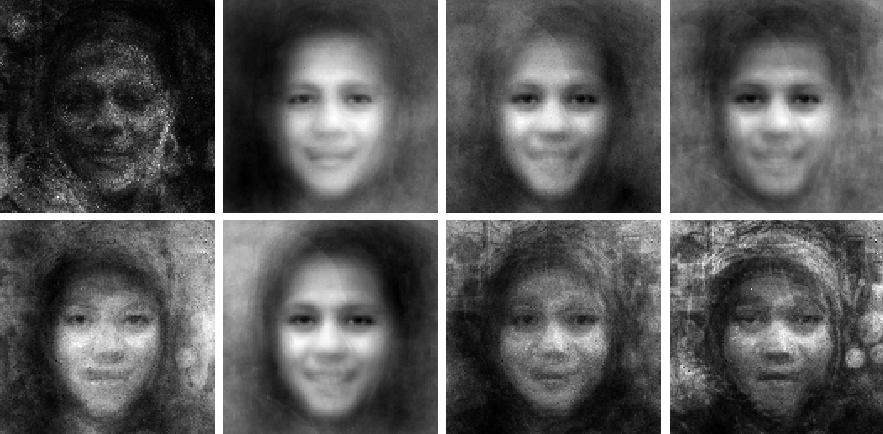
\includegraphics[width=\textwidth]{fig/vae/ffhq_epoch1000}
        \caption{Epoch 1000}
    \end{subfigure}
    ~
    \begin{subfigure}[b]{0.45\textwidth}
         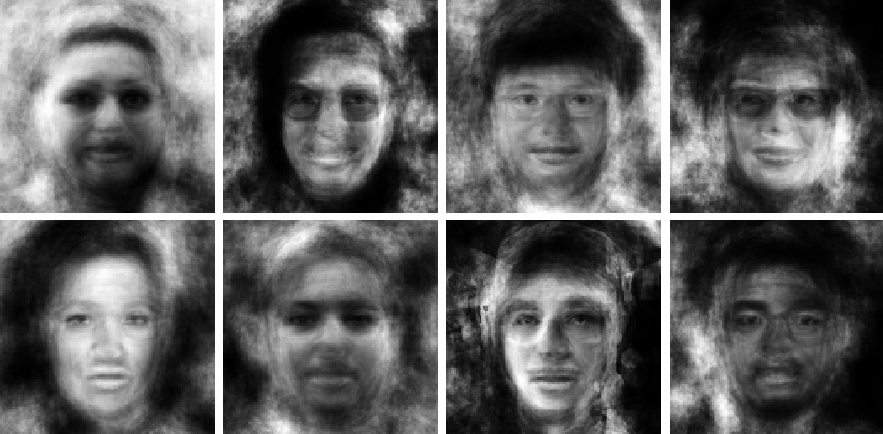
\includegraphics[width=\textwidth]{fig/vae/ffhq_epoch2000}
        \caption{Epoch 2000}
    \end{subfigure}

    \begin{subfigure}[b]{\textwidth}
         \includegraphics[width=\textwidth]{fig/vae/ffhq_epoch4000}
        \caption{Epoch 4000}
    \end{subfigure}
    \caption{Samples from Variational Autoencoder  during training on a black and white version of  the FFHQ dataset}
    \label{vaq-bwffhq-samples}
\end{figure}

\begin{figure}[h!]
    \centering
    \begin{subfigure}[b]{0.45\textwidth}
        \includegraphics[width=\textwidth]{fig/vae/ffhq_epoch50color}
        \caption{Epoch 50}
    \end{subfigure}
    ~
    \begin{subfigure}[b]{0.45\textwidth}
         \includegraphics[width=\textwidth]{fig/vae/ffhq_epoch400color}
        \caption{Epoch 400}
    \end{subfigure}

    \begin{subfigure}[b]{0.45\textwidth}
         \includegraphics[width=\textwidth]{fig/vae/ffhq_epoch1000color}
        \caption{Epoch 1000}
    \end{subfigure}
    ~
    \begin{subfigure}[b]{0.45\textwidth}
         \includegraphics[width=\textwidth]{fig/vae/ffhq_epoch2000color}
        \caption{Epoch 2000}
    \end{subfigure}

    \begin{subfigure}[b]{\textwidth}
         \includegraphics[width=\textwidth]{fig/vae/ffhq_epoch4000color}
        \caption{Epoch 4000}
    \end{subfigure}
    \caption{Samples from Variational Autoencoder during training on the color version of the FFHQ dataset}
    \label{vaq-ffhq-samples}
\end{figure}



%% DCGAN
\begin{figure}
    \centering
    \begin{subfigure}[b]{0.45\textwidth}
        \includegraphics[width=\textwidth]{fig/dcgan/ffhq/epoch0}
        \caption{Epoch 0}
    \end{subfigure}
    ~
    \begin{subfigure}[b]{0.45\textwidth}
        \includegraphics[width=\textwidth]{fig/dcgan/ffhq/epoch200}
        \caption{Epoch 200}
    \end{subfigure}

    \begin{subfigure}[b]{0.45\textwidth}
        \includegraphics[width=\textwidth]{fig/dcgan/ffhq/epoch2000}
        \caption{Epoch 2000}
    \end{subfigure}
    ~
    \begin{subfigure}[b]{0.45\textwidth}
        \includegraphics[width=\textwidth]{fig/dcgan/ffhq/epoch4000}
        \caption{Epoch 4000}
    \end{subfigure}

    \begin{subfigure}[b]{\textwidth}
        \includegraphics[width=\textwidth]{fig/dcgan/ffhq/epoch10000}
        \caption{Epoch 100000}
    \end{subfigure}
    \caption{Samples from DCGAN during training on the FFHQ dataset}
    \label{dcgan-ffhq-samples}
\end{figure}


\begin{figure}[h!]
\centering
\begin{subfigure}[b]{0.45\textwidth}
\includegraphics[width=\textwidth]{fig/dcgan/caltech/loss}
\caption{ Caltech Dataset}
\end{subfigure}
\begin{subfigure}[b]{0.45\textwidth}
\includegraphics[width=\textwidth]{fig/dcgan/ffhq/loss}
\caption{FFHQ  Dataset}
\end{subfigure}
\caption{Loss and accuracy of the discriminator during training}
\end{figure}

\begin{figure}
    \centering
    \begin{subfigure}[b]{0.45\textwidth}
        \includegraphics[width=\textwidth]{fig/dcgan/caltech/epoch0}
        \caption{Epoch 0}
    \end{subfigure}
    ~
    \begin{subfigure}[b]{0.45\textwidth}
        \includegraphics[width=\textwidth]{fig/dcgan/caltech/epoch200}
        \caption{Epoch 200}
    \end{subfigure}

    \begin{subfigure}[b]{0.45\textwidth}
        \includegraphics[width=\textwidth]{fig/dcgan/caltech/epoch2000}
        \caption{Epoch 200}
    \end{subfigure}
    ~
    \begin{subfigure}[b]{0.45\textwidth}
        \includegraphics[width=\textwidth]{fig/dcgan/caltech/epoch4000}
        \caption{Epoch 4000}
    \end{subfigure}

    \begin{subfigure}[b]{\textwidth}
        \includegraphics[width=\textwidth]{fig/dcgan/caltech/epoch10000}
        \caption{Epoch 10000}
    \end{subfigure}
    \caption{Samples from DCGAN during training on the Caltech dataset}
    \label{dcgan-caltech-samples}
\end{figure}



\end{document}
